\chapter{Syntax}

Es gibt hierbei mehrere Punkte zu beachten. Der wichtigste ist wahrscheinlich, dass man seinen Stil w�hlt und diesen immer beibeh�lt.
Jedoch sollten auch folgende Punkte beachtet werden:\\

\begin{itemize}
  \item KEIN DENGLISCH: \\
  			Es sollte auf keinen Fall Deutsch und Englisch vermischt werden. So z.B. kann man anstatt dem sehr h�ufig verwendeten englischen Begriff "`file"'
  			ohne weiteres den deutschen "`Datei"' verwenden. Trotzdem ist zu beachten, dass dies manchmal nicht m�glich sein kann, da es sich um einen 							einzigartigen Begriff wie z.B. "`Programm-Code"' handelt.
  \item EINHEITLICHE SCHREIBWEISE:\\
  			Immer einheitlich schreiben. Nie bei Begriffen mehrere verschiedene Bezeichnungen oder Buchstabengr��en verwenden, wie z.B.:\\
  			Matlab - MatLab - MATLAB\\
  			Hier kann man gerade bei solch speziellen Ausdr�cken, die meistens auch noch l�nger sind (z.B.: MATLAB/Simulink) durch einen einfachen Trick
  			Abhilfe schaffen. Man definiert diese Zeichenkette als Befehl, wodurch die einheitliche Schreibweise gew�hrleistet ist.\\
  			z.B.: \textit{$\setminus$newcommmand\{$\setminus$MS \}\{MATLAB/Simulink\}}
  \item KEINE WORTWIEDERHOLUNGEN\\
  			Bitte auf ein angenehm lesbares Deutsch achten.
  \item KEIN KONJUNKTIV\\
  			Die Diplomarbeit ist eine wissenschaftliche Arbeit, in der der Konjunktiv nichts verloren hat.
  \item KEINE "`WIR"'-FORM\\
  			Ebenso d�rfen in einer wissenschaftlichen Arbeit keine Personal- Possessiv- oder Reflexivpronomina verwendet werden.\\
  			(z.B. ich, du, ... mein, dein, .... mich, dich, ...)
  			Sehr wohl kann das Indefinitpronomen "`man"' verwendet werden, vom h�ufigen Gebrauch ist jedoch abzuraten.
  \item EIGEN- UND FIRMENNAMEN KURSIV (mit dem Befehl "`textsc{}"')
  			
  \item REFERENZIERUNG\\
  			Die W�rter "`Tabelle"' und "`Gleichung"' sollten am Satzanfang ausgeschrieben, innerhalb eines Satzes sollten die Abk�rzungen "`Tab."' 								und "`Gl."' verwendet werden.
  \item BINDESTRICHE
  			Mit einem zus�tzlichen Leerzeichen bei Gegen�berstellungen, ohne bei Wortbindungen. z.B.:\\
  			Arm - Bein\\
  			PD-Regelung
  \item MATRIZEN UND VEKTOREN FETT\\
  			Die Schreibweise sollte an das Robotik-Skriptum angelehnt werden !!
  \item MATHEMATISCHE FORMELN UND ZEICHEN\\
  			... geh�ren auch IM TEXT im "`Math-Modus"' geschrieben !! So zum Beispiel sollte die Minimalkoordinate "`q"' im Text als $q$ angef�hrt werden.
\end{itemize}



\section{Einige LaTeX - Beispiele}

\subsection{Einbinden von Bildern}

Die Erfahrung hat gezeigt, dass sich "`.eps"'-Graphiken am besten eignen. Um Skizzen  anzufertigen sollte ein Vektorgrafikprogramm, wie z.B. \textsc{Corel Designer}, verwendet werden. Rastergrafiken k�nnen innerhalb der "`eps"'-Dateien als Bitmap mit "`jpg"'-Komprimierung eingef�gt werden. Somit entstehen scharfe Grafiken. Unscharfe Grafiken aufgrund der Anwendung von Rastergrafiken ("`bmp"' oder "`jpg"') werden nicht akzeptiert! Um eine "`.pdf"'-Datei zu erstellen, sollte beim Ausgabeprofil "`LaTeX => PS => PDF"' gew�hlt werden.

\begin{figure}[H]
	\centering	
		\psfragscanon		
		\psfrag{P}[c][c]{$\hat{P}$}
    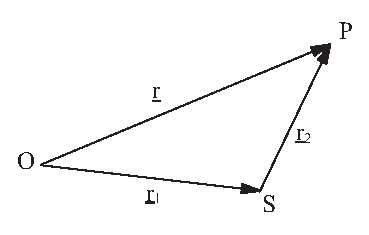
\includegraphics[width=0.4\textwidth,angle=0]{dreieck.eps}		
		 \caption{Ein Beispiel eines Bildes}
		 \label{Beispiel}
\end{figure}
Man kann anschlie�end sehr einfach auf das entsprechende Bild referenzieren, wie zum Beispiel auf dieses Bild mit der Bezeichnung Bild \ref{Beispiel}.\\
Die Schriftgr��e sowie der Schriftstyle m�ssen mit dem Text im Dokument �bereinstimmen. Entweder verwendet man im Grafikprogramm eine geeignete Schrift
oder man verwendet bei eps - Grafiken das "`psfrag"'-Packet zum Ersetzen der Schrift ( $\hat{P}$ in Bild \ref{Beispiel} wurde mit "`psfrag"' erzeugt).\\
An und f�r sich sollte auf alle Grafiken im Text referenziert sein.

\subsection{Mathematische Formeln}

Hier sei nur ein kurzes Beispiel gezeigt, in den entsprechenden B�chern gibt es ausf�hrlichste Beschreibungen gerade zum Editieren von Formeln.

\begin{eqnarray*}
_{k}\,\mathbf{J} &=&\int\limits_{K}\left( 
\begin{array}{ccc}
0 & -z & y \\ 
z & 0 & -x \\ 
-y & x & 0%
\end{array}%
\right) \,\left( 
\begin{array}{ccc}
0 & z & -y \\ 
-z & 0 & x \\ 
y & -x & 0%
\end{array}%
\right) \,dm \\
_{k}\,\mathbf{J} &=&\int\limits_{K}\left( 
\begin{array}{ccc}
y^{2}+z^{2} & -x\,y & -x\,z \\ 
-x\,y & x^{2}+z^{2} & -y\,z \\ 
-x\,z & -y\,z & x^{2}+y^{2}%
\end{array}%
\right) \,dm 
\end{eqnarray*}


Jede Formel muss im Text eingef�gt sein. Das Ganze muss wie ein Buch lesbar sein. Jeder Satz endet mit einem Punkt (auch wenn am Ende eine Formel steht!).\\
\underline{Bsp.:} Der Gelenkpunkt hat dabei die Koordinaten
\begin{equation} 
	_i \mathbf{r}_{oi}=\sum \mathbf{A}_{ip}\ _p\mathbf{r}_{pj}
\end{equation}
und die Orientierung
\begin{equation} 
	\mathbf{A}_{oi} = \Pi \mathbf{A}_{pj}.
\end{equation}
